\documentclass[../main.tex]{subfiles}
\graphicspath{{\subfix{../images/}}}
\begin{document}

Our nutrition is composed of multiple basic building blocks, which each in turn have very different
tasks to perform in our body.

the beginning and end of a healthy nutrition is to combine the basic building blocks in a sensible way and it helps us
to maintain our body to the be lean, healthy and full of power into a high age.

These basic building blocks of our food are:
\begin{itemize}
\item Water
\item Proteins
\item Fats (lipids)
\item Carbohydrates (sugar, starch)
\item Vital substances
\item Fibers
\end{itemize}

\begin{table}[htb!]
  \centering
  \begin{tabular}{lcccc}
    \textbf{Building Block} & \textbf{kJ/g} & \textbf{kcal/g} & \textbf{kJ/oz} & \textbf{kcal/oz} \\
    Proteins & 17 & 4 & 482 & 113 \\
    Fats & 37 & 9 & 1049 & 255 \\
    Carbohydrates & 17 & 4 & 482 & 113 \\
  \end{tabular}
  \caption{Energy content of the different building blocks of our food}
\end{table}

\section{Water}

\begin{figure}[htb!]
  \centering

\includegraphics[width=5cm]{GlassWater.eps}
  \caption{A glass of water~\cite{GlassWater}}
\end{figure}



Water doesn't contain any nutrients, but nevertheless is water of the biggest importance for the human body.
Without water, there's no life.
The human body consists our of about 60\% water (a newborn even up to 75\%).
Roughly 60\% of that water is found in the intracellular space (inside the cells).
The rest is in between the cells in the form of interstitial fluids (between the cells),
like blood plasma, lymph, urine, saliva, digestion fluids, tear liquid, nose secretes and sweat.


In the human organism, water mainly serves:
\begin{itemize}
\item to cover the needs of fluids in cells and tissues,
\item as a solvent and medium of transportation for nutrients, enzymes, hormones and so on,
\item to excrete metabolism end products over the urine,
\item to regulate the body temperature.
\end{itemize}

\subsection{How much Water does a Human Being Need?}

During a day, the human body looses\index{water consumption} 2--2.5 liters (8\sfrac{1}{2}\ -- 10\sfrac{1}{2}\ cups) of water, of which:
\begin{itemize}
\item 1.0 -- 1.5 L (4\sfrac{1}{4}\ -- 6\sfrac{1}{4}\ cups) through the urine
\item 0.4 -- 1.0 L (1\sfrac{3}{4}\ -- 4\sfrac{1}{4}\ cups) through respiration
\item 0.1 -- 0.5 L (3\sfrac{1}{2}\ fl.oz. -- 2\sfrac{1}{8}\ cups) over the skin, through sweat
  \item 0.1 -- 0.2 L (3\sfrac{1}{2}\ -- 7 fl.oz.) through feces
  \end{itemize}

  This loss of water has to be added back to our body on a daily base, through drinking and eating.
  For a healthy, barely physical active person, that means a daily fluid intake of about 30 -- 35 mL of fluids per kg (0.45 -- 0.54 fl.oz./lbs) body weight.
  A person who weights 70 kg (154 lbs) therefore needs a fluid supply of 2.0 -- 2.5 L (8\sfrac{1}{2}\ -- 10\sfrac{1}{2} cups) per day.
  Out of this amount, about 0.5 -- 1 L (2\sfrac{1}{8}\ -- 4\sfrac{1}{4} cups) fluids will be supplied through food (veggies, fruits, \ldots).
  This results then in the recommended amount of drinking about 1 -- 2 L (one to two quarts) of fluids a day.

  Please consider, that the water usage also depends on the outside temperature, physical activity levels and the state of health.
  When it's hot, under heavy physical labor or sport, sweating will cool down the body and
  in case of disease (fever, diarrhea, vomiting) the body will also loose a lot of additional water.
  All these losses need to be compensated with additional fluid intake.

  \subsection{Is Water the Best Drink?}

  As drinks counts foods, which pretty much only furnish water to our body. 
  Fruit and veggie juices, milk, yogurt drinks and soft drinks deliver next to water plenty of nutrients and energy and  don't really count as drinks.
  Alcoholic drinks are non--essential food items, stimulants and are very bad at hydrating our body.
  On top of that, they are delivering a lot of unwanted energy (about 7 kcal/g, roughly 200 kcal per oz.).

% Swiss tap water - US tap water?
  
  Pure water is by far the best and cheapest drink. Tap water, depending on location filtered, is the best option to hydrate.
  In order to change things up, can water be flavored in different ways:
  \begin{itemize}
  \item Fruit or herbal tea
  \item Black or green tea, coffee\footnote{See special drinks and foods in the section \ref{SpecialFoods}, page~\pageref{SpecialFoods}.}
  \item Broth
    \item Lemon water (juice of one lemon for one Liter (quart) of water)
  \end{itemize}

  People who are depended on bottled water, should preferably choose still water.
  The carbonation leeches vital oxygen from our body and adds unnecessary acids to our system.

  \subsection[Drinking Too Little, Too Much or the Wrong Drinks]{People Who Drink Not Enough, Too Much or the Wrong Things Risk their Health}

  Humans can survive multiple weeks without food, but without fluids only three days.
  Already a loss of fluids of 1\% or our body weight leads to the first symptoms like head ache, difficulties focusing and thirst.
  Being thirsty already indicates a lack in fluids.
  With advances age, the thirst signal decreases, which in turn is the reason that older people often don't drink enough.
  Among other effects, this leads to:
  \begin{itemize}
  \item higher viscosity of the blood, with the danger of thrombosis and a decreased oxygen supply of the organs
  \item dry skin, which is easier to be hurt
  \item drier mucous membranes, which are more susceptible to infections
    \item constipation, through excessive thickening of the feces
    \end{itemize}

    An excessive intake in fluids also can threaten the physical productivity and in excess even get dangerous.
    But the biggest danger comes from the many calories, if soft drinks or alcoholic drinks get consumed in excess. 

 
\vspace{5mm}
\noindent
\begin{fminipage}{\textwidth}
  \textbf{Profile Water}
  \begin{itemize}
  \item The human body consists of 60 \% of water and a human can only survive three days without water intake
  \item Water is vital for humans, it transports nutrients, enzymes and hormones to the cells; it helps the excretion of harmful substances and the regulation of the body temperature
  \item Water is free of calories and doesn't deliver energy to the body
  \item We need about 2 -- 2.5 L (8\sfrac{1}{2}\ -- 10\sfrac{1}{2}\ cups) of fluids a day, thereof 1 -- 2 L (1 -- 2 quarts) in the form of water
    \item Preferably pure water or mineral water without carbonation
  \end{itemize}
\end{fminipage}

\section{Proteins}

\begin{figure}[htb!]
\centering
  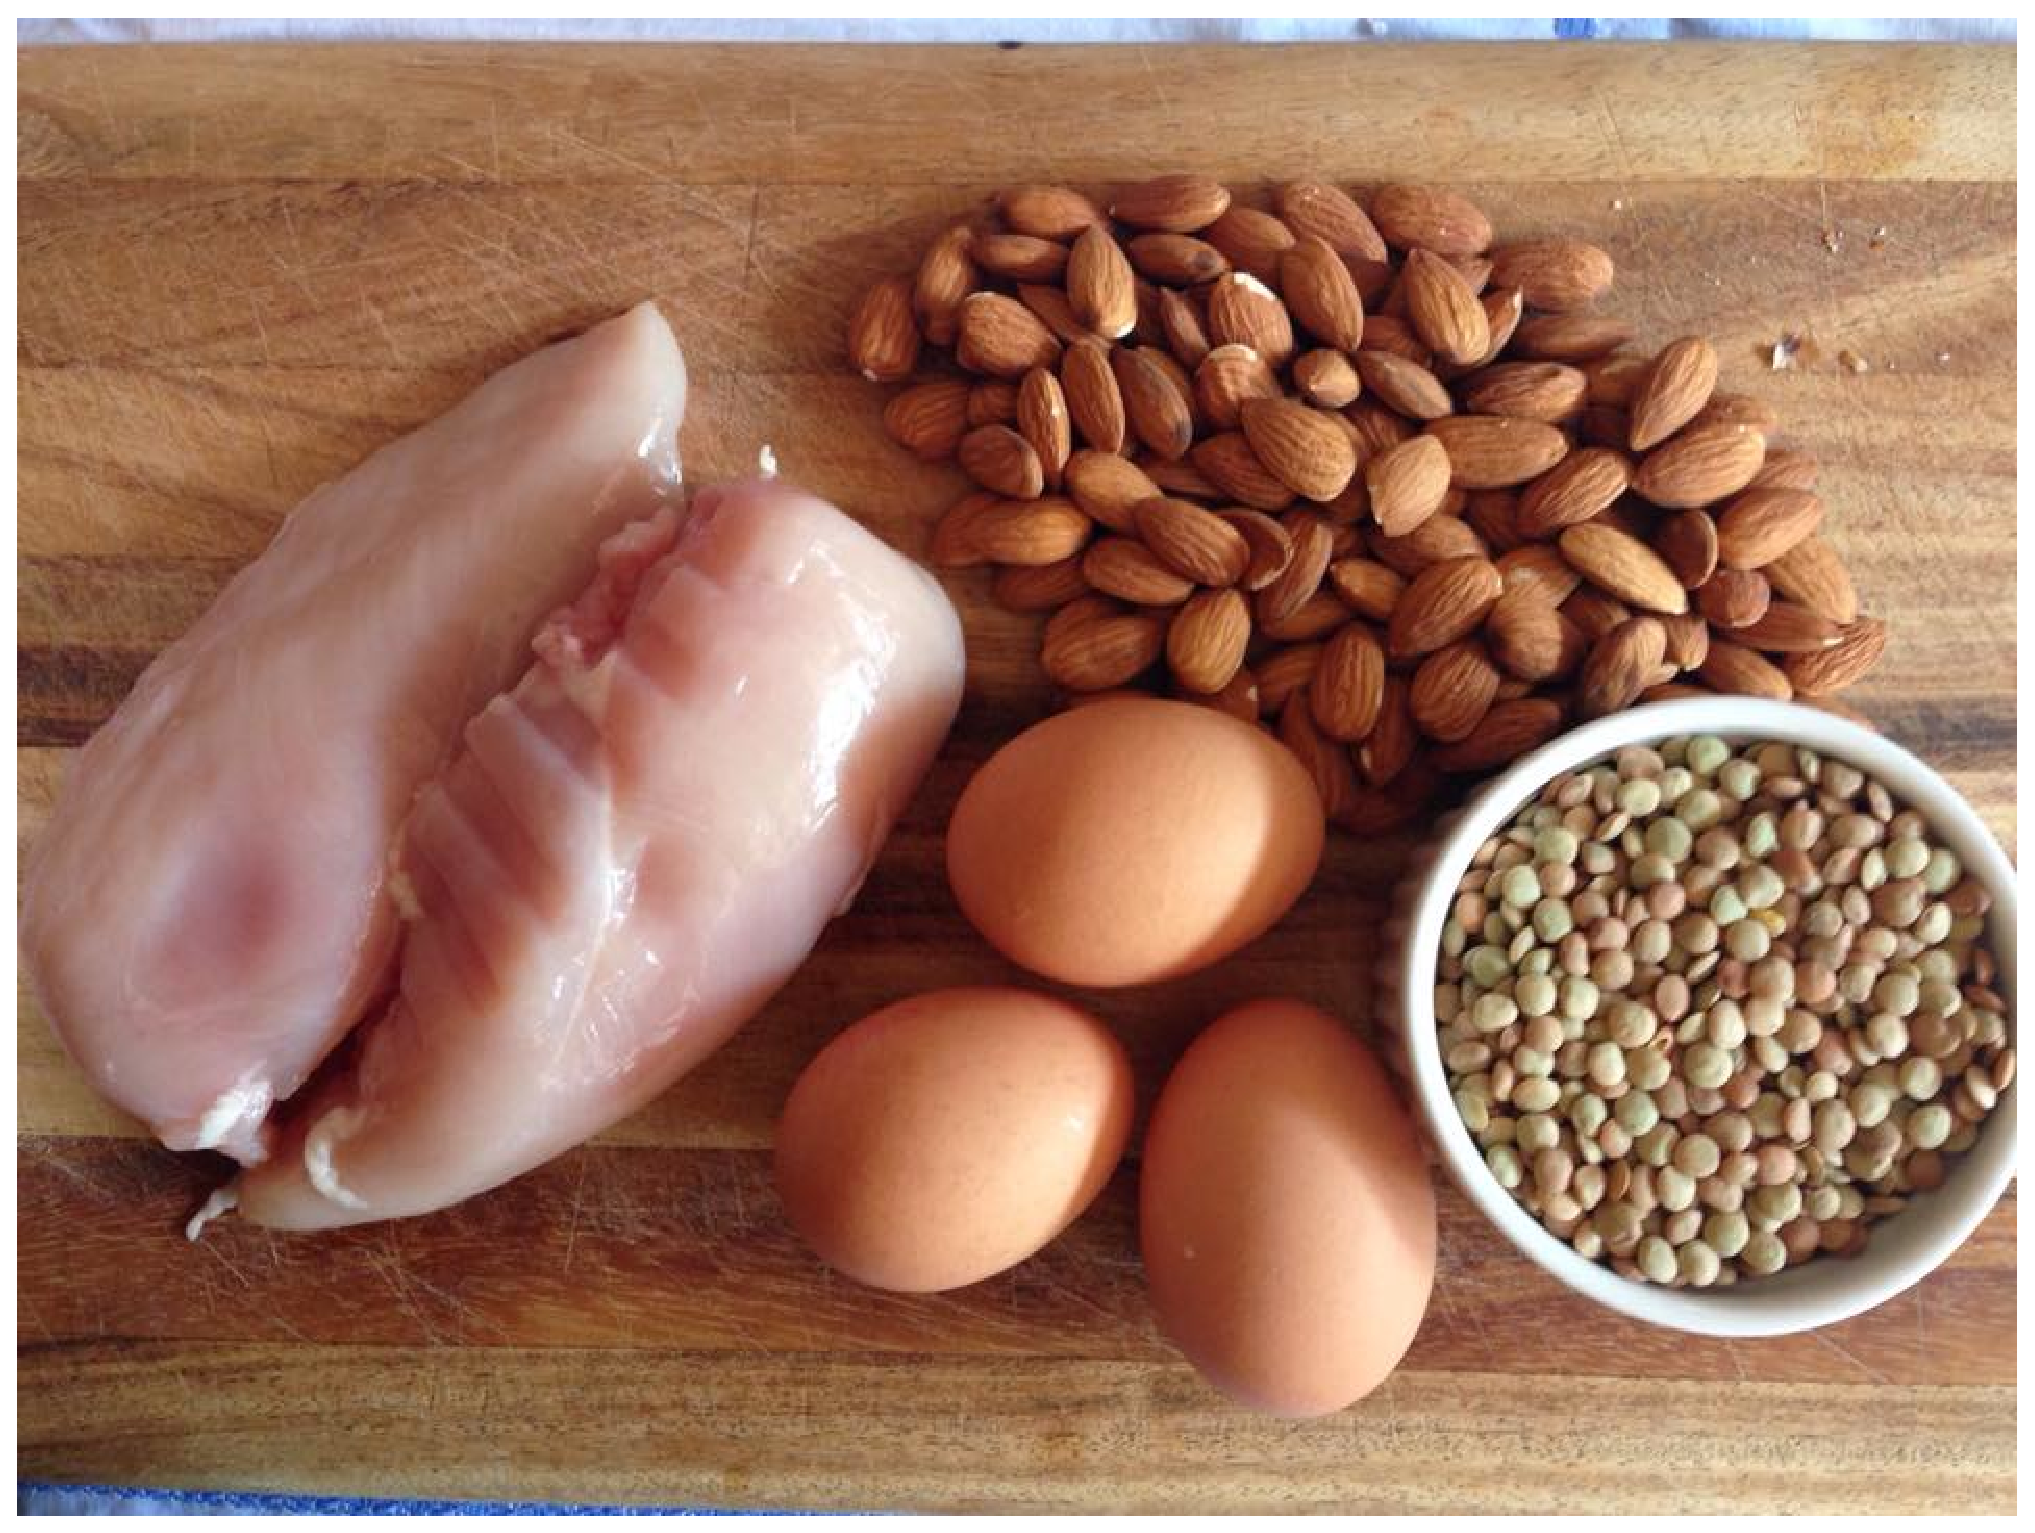
\includegraphics[width=7cm]{Protein-rich_Foods}
  \caption{Protein rich foods\cite{Proteins}}
  % It says from wikipedia https://upload.wikimedia.org/wikipedia/commons/e/e8/Protein-rich_Foods.jpg
\end{figure}

First and foremost, are proteins building blocks to build up our bodies.
Proteins are the basic building blocks of every single one of our cells, of muscles, connective tissue, skin,
blood, internal organs, hormones and enzymes.
Given that the body cells get constantly renewed and built up again and again, we humans require a constant supply of proteins.
A lack in proteins can lead to a dismantlement of important parts of the body.
But too much proteins isn't good either.
Excessive proteins can only be stored in our bodies to a very limited amount.
So superfluous proteins, or their degradation products urea and uric acid, have to be excreted over the kidneys.
This in turn can overburden the kidneys and lead to rheumatism and gout.
Only secondarily are proteins used for energy.
As carbohydrates, they deliver 4 kcal or 17 kJ of energy per gramm (113 kcal or 482 kJ per oz.).

Proteins have very different roles in our body. A selection:
\begin{itemize}
\item in the form of collagen (about \sfrac{1}{3} of the body's proteins), they build up the structure of the skin, connective tissue and the bones
\item in our muscles, myosine and actine change their shapes and by doing doing lead to contractions of the muscles and allow us to move
\item enzymes organize and execute the biocatalytic functions, that means they allow  and control specific (bio)chemical reactions in our body
\item as transport proteins, they organize the transport of vital substances like for instance hemoglobin, which organizes the transport of oxygen in the blood stream
\item as antibodies, they serve to combat infections
  \item as reserves, they serve the body as energy supply in the case of hunger.
  \end{itemize}

  \subsection{The Structure of Proteins}
  
\end{document}